% Options for packages loaded elsewhere
\PassOptionsToPackage{unicode}{hyperref}
\PassOptionsToPackage{hyphens}{url}
\PassOptionsToPackage{dvipsnames,svgnames,x11names}{xcolor}
%
\documentclass[
  b5paper,
  DIV=11,
  numbers=noendperiod]{scrreprt}

\usepackage{amsmath,amssymb}
\usepackage{iftex}
\ifPDFTeX
  \usepackage[T1]{fontenc}
  \usepackage[utf8]{inputenc}
  \usepackage{textcomp} % provide euro and other symbols
\else % if luatex or xetex
  \usepackage{unicode-math}
  \defaultfontfeatures{Scale=MatchLowercase}
  \defaultfontfeatures[\rmfamily]{Ligatures=TeX,Scale=1}
\fi
\usepackage{lmodern}
\ifPDFTeX\else  
    % xetex/luatex font selection
\fi
% Use upquote if available, for straight quotes in verbatim environments
\IfFileExists{upquote.sty}{\usepackage{upquote}}{}
\IfFileExists{microtype.sty}{% use microtype if available
  \usepackage[]{microtype}
  \UseMicrotypeSet[protrusion]{basicmath} % disable protrusion for tt fonts
}{}
\makeatletter
\@ifundefined{KOMAClassName}{% if non-KOMA class
  \IfFileExists{parskip.sty}{%
    \usepackage{parskip}
  }{% else
    \setlength{\parindent}{0pt}
    \setlength{\parskip}{6pt plus 2pt minus 1pt}}
}{% if KOMA class
  \KOMAoptions{parskip=half}}
\makeatother
\usepackage{xcolor}
\setlength{\emergencystretch}{3em} % prevent overfull lines
\setcounter{secnumdepth}{3}
% Make \paragraph and \subparagraph free-standing
\ifx\paragraph\undefined\else
  \let\oldparagraph\paragraph
  \renewcommand{\paragraph}[1]{\oldparagraph{#1}\mbox{}}
\fi
\ifx\subparagraph\undefined\else
  \let\oldsubparagraph\subparagraph
  \renewcommand{\subparagraph}[1]{\oldsubparagraph{#1}\mbox{}}
\fi


\providecommand{\tightlist}{%
  \setlength{\itemsep}{0pt}\setlength{\parskip}{0pt}}\usepackage{longtable,booktabs,array}
\usepackage{calc} % for calculating minipage widths
% Correct order of tables after \paragraph or \subparagraph
\usepackage{etoolbox}
\makeatletter
\patchcmd\longtable{\par}{\if@noskipsec\mbox{}\fi\par}{}{}
\makeatother
% Allow footnotes in longtable head/foot
\IfFileExists{footnotehyper.sty}{\usepackage{footnotehyper}}{\usepackage{footnote}}
\makesavenoteenv{longtable}
\usepackage{graphicx}
\makeatletter
\def\maxwidth{\ifdim\Gin@nat@width>\linewidth\linewidth\else\Gin@nat@width\fi}
\def\maxheight{\ifdim\Gin@nat@height>\textheight\textheight\else\Gin@nat@height\fi}
\makeatother
% Scale images if necessary, so that they will not overflow the page
% margins by default, and it is still possible to overwrite the defaults
% using explicit options in \includegraphics[width, height, ...]{}
\setkeys{Gin}{width=\maxwidth,height=\maxheight,keepaspectratio}
% Set default figure placement to htbp
\makeatletter
\def\fps@figure{htbp}
\makeatother

\usepackage{libertine}
\addtokomafont{disposition}{\rmfamily}
\renewcommand{\ttdefault}{clmt}
\providecommand{\ped}[1]{_\textrm{#1}}
\providecommand{\ap}[1]{^\textrm{#1}}
\providecommand{\app}[1]{^\textrm{#1}}

\providecommand*{\angs}{\smash{\mathrm{\ring A}}}
\providecommand*{\celsius}{\mathrm{~\circ C}}
\providecommand*{\micro}{\mu}

\providecommand*{\unit}[1]{\textrm{\,#1}}


\providecommand{\E}{\mathrm{e}}
\providecommand{\I}{\mathrm{i}}
\providecommand{\sfrac}[2]{^{#1}/_{#2}}

\providecommand{\conc}[1]{\left[\mathrm{#1}\right]}


\providecommand{\command}[1]{\textsl{#1}}
\providecommand{\out}[1]{\begin{verbatim}#1\end{verbatim}}


\providecommand{\diff}{\mathrm{d}\,}


\providecommand*{\deriv}[3][]{% arguments: order of the derivative(optional), function, variable
	\frac{\diff^{#1}#2}{\diff #3^{#1}}}
\providecommand*{\pderiv}[3][]{% arguments: order of the derivative(optional), function, variable
	\frac{\partial^{#1}#2}
		{\partial #3^{#1}}}
  
\renewcommand{\vec}[1]{{\boldsymbol #1}}

\providecommand{\cov}[2]{\mathrm{Cov}\!\left(#1, #2\right)}
\providecommand{\var}[1]{\mathrm{Var}\!\left(#1\right)}

\providecommand{\mean}[1]{\overline{#1}}

\providecommand{\sd}[1]{\sigma\left(#1\right)}
\providecommand{\ev}[1]{\mathbb{E}\!\left(#1\right)}
\providecommand{\pr}[1]{\textrm{Pr}\!\left(#1\right)}

\KOMAoption{captions}{tableheading}
\makeatletter
\@ifpackageloaded{bookmark}{}{\usepackage{bookmark}}
\makeatother
\makeatletter
\@ifpackageloaded{caption}{}{\usepackage{caption}}
\AtBeginDocument{%
\ifdefined\contentsname
  \renewcommand*\contentsname{Inhoudsopgave}
\else
  \newcommand\contentsname{Inhoudsopgave}
\fi
\ifdefined\listfigurename
  \renewcommand*\listfigurename{Lijst van figuren}
\else
  \newcommand\listfigurename{Lijst van figuren}
\fi
\ifdefined\listtablename
  \renewcommand*\listtablename{Lijst van tabellen}
\else
  \newcommand\listtablename{Lijst van tabellen}
\fi
\ifdefined\figurename
  \renewcommand*\figurename{Figuur}
\else
  \newcommand\figurename{Figuur}
\fi
\ifdefined\tablename
  \renewcommand*\tablename{Tabel}
\else
  \newcommand\tablename{Tabel}
\fi
}
\@ifpackageloaded{float}{}{\usepackage{float}}
\floatstyle{ruled}
\@ifundefined{c@chapter}{\newfloat{codelisting}{h}{lop}}{\newfloat{codelisting}{h}{lop}[chapter]}
\floatname{codelisting}{Listing}
\newcommand*\listoflistings{\listof{codelisting}{Lijst van listings}}
\makeatother
\makeatletter
\makeatother
\makeatletter
\@ifpackageloaded{caption}{}{\usepackage{caption}}
\@ifpackageloaded{subcaption}{}{\usepackage{subcaption}}
\makeatother
\ifLuaTeX
\usepackage[bidi=basic]{babel}
\else
\usepackage[bidi=default]{babel}
\fi
\babelprovide[main,import]{dutch}
% get rid of language-specific shorthands (see #6817):
\let\LanguageShortHands\languageshorthands
\def\languageshorthands#1{}
\ifLuaTeX
  \usepackage{selnolig}  % disable illegal ligatures
\fi
\usepackage{bookmark}

\IfFileExists{xurl.sty}{\usepackage{xurl}}{} % add URL line breaks if available
\urlstyle{same} % disable monospaced font for URLs
\hypersetup{
  pdftitle={Kwantitatieve Biologie},
  pdfauthor={Vakgroep Biologie, Universiteit Utrecht},
  pdflang={nl},
  colorlinks=true,
  linkcolor={blue},
  filecolor={Maroon},
  citecolor={Blue},
  urlcolor={Blue},
  pdfcreator={LaTeX via pandoc}}

\title{Kwantitatieve Biologie}
\author{Vakgroep Biologie, Universiteit Utrecht}
\date{2024-06-20}

\begin{document}
\maketitle

\renewcommand*\contentsname{Inhoudsopgave}
{
\hypersetup{linkcolor=}
\setcounter{tocdepth}{2}
\tableofcontents
}
\bookmarksetup{startatroot}

\chapter{Inleiding}\label{inleiding}

\part{Programmeren in R}

\begin{figure}

\centering{


\includegraphics{Programmeren/figuren/AI_R.jpeg}

}

\caption{\label{fig-AI_R}Programmeren in R voor biologien, illustratie
gegenereerd door AI. (DALL-E 3, Maart 2024)}

\end{figure}%

\chapter{Wat is R?}\label{wat-is-r}

\part{Basiswiskunde}

\begin{figure}

\centering{

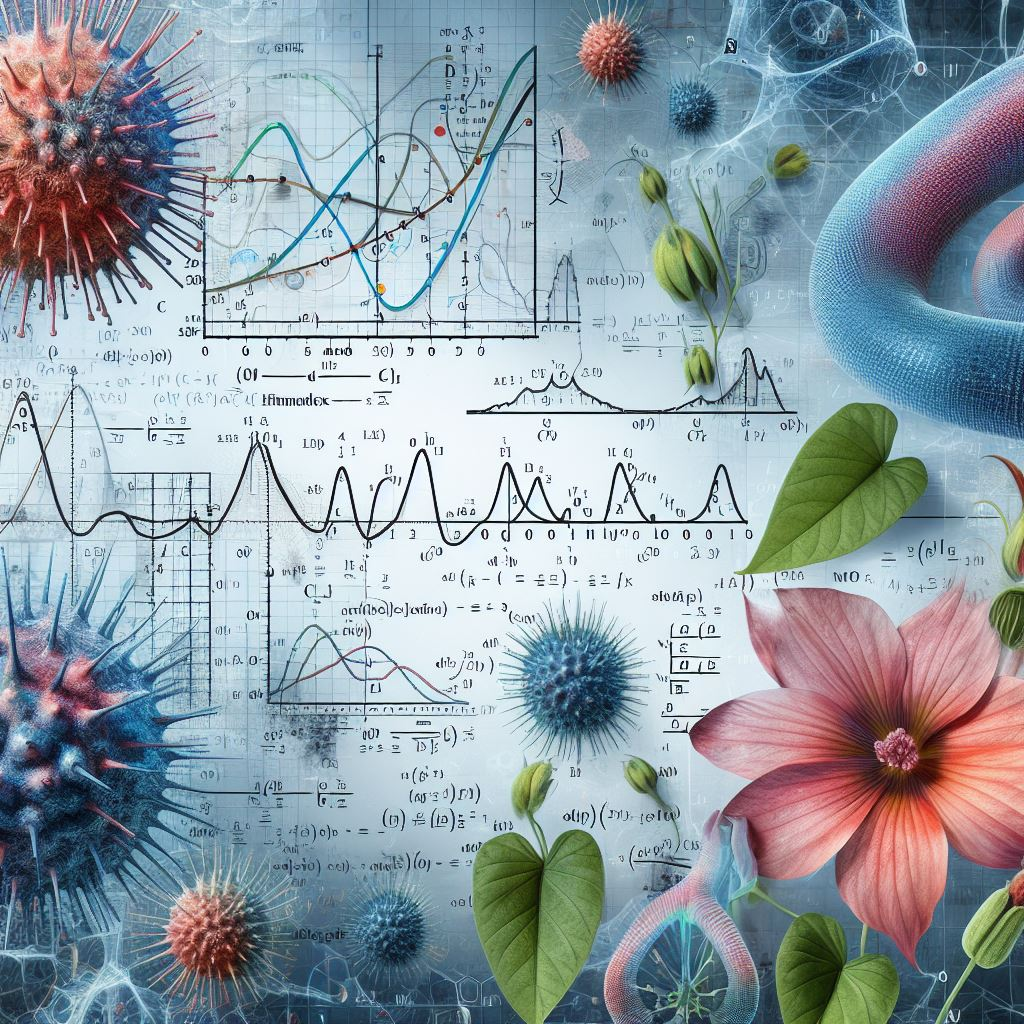
\includegraphics{Wiskunde/figuren/AI_mathematics.jpeg}

}

\caption{\label{fig-AI_mathematics}Wiskunde in de biologie; illustratie
gegenereerd door AI. (DALL-E 3, maart 2024)}

\end{figure}%

\chapter{Breuken}\label{breuken}

\part{Biologische modellering}

\begin{figure}

\centering{

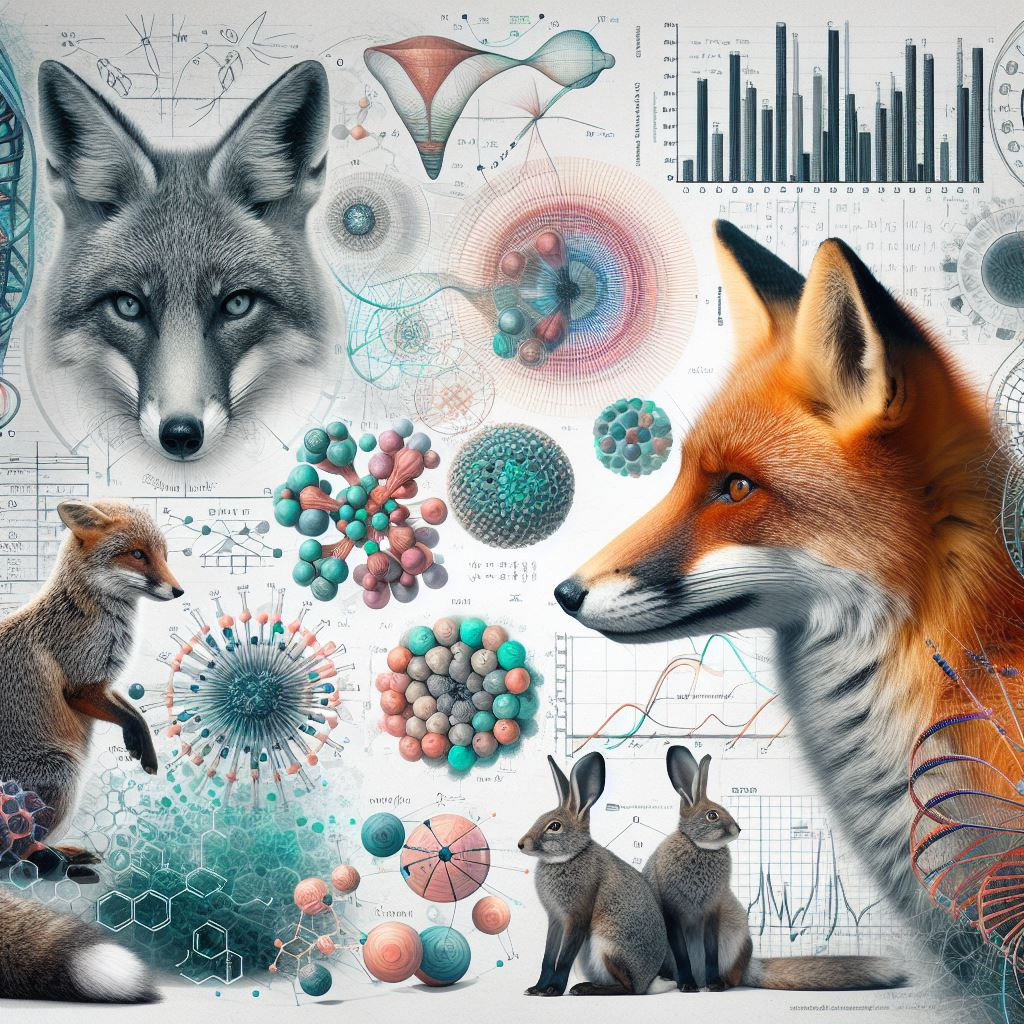
\includegraphics{Modellering/figuren/AI_models.jpeg}

}

\caption{\label{fig-AI_models}Modellering in de biologie, illustratie
gegenereerd door AI. (DALL-E 3, maart 2024)}

\end{figure}%

\begin{figure}[H]

{\centering 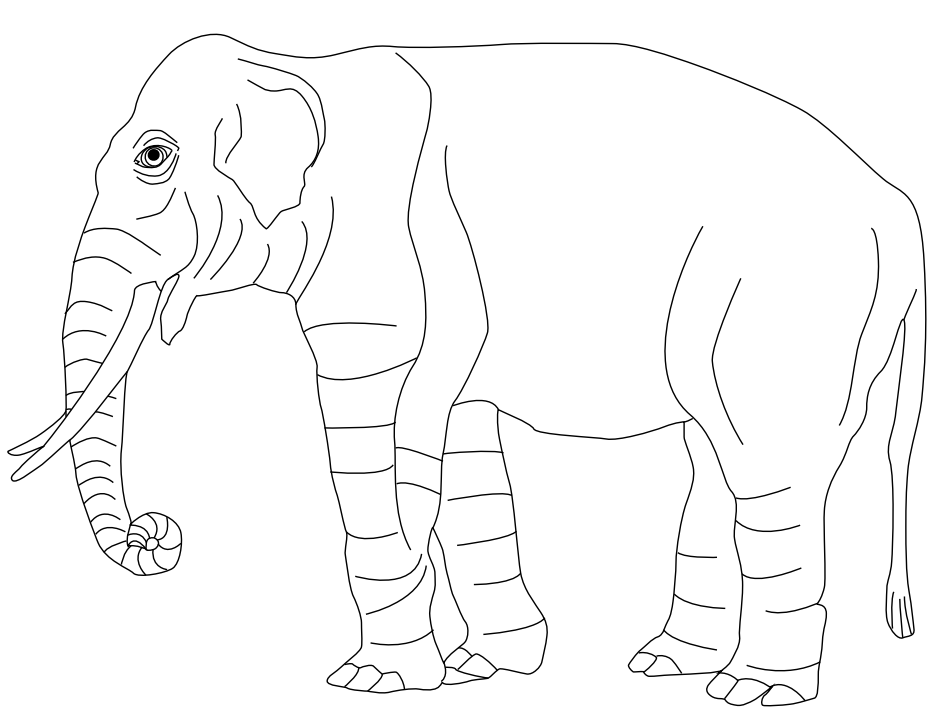
\includegraphics[width=4in,height=\textheight]{Modellering/../figuren/elephant.png}

}

\caption{Ga naar \url{https://tbb.bio.uu.nl/bvd/simulations/australia/}
voor de simulatie.}

\end{figure}%

\chapter{Modellen in de biologie}\label{modellen-in-de-biologie}

\part{Statistiek voor biologen}

\begin{figure}

\centering{

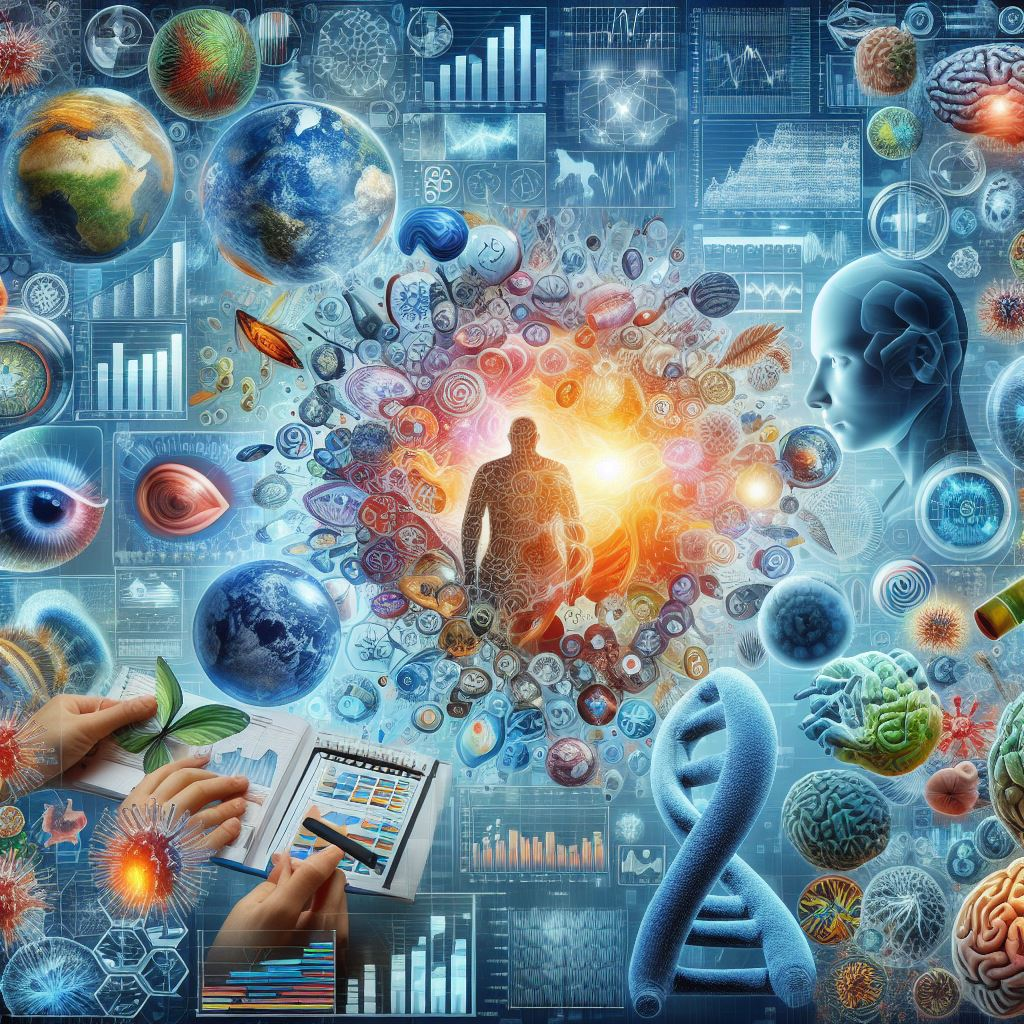
\includegraphics{Statistiek/figuren/AI_statistics.jpeg}

}

\caption{\label{fig-AI_statistics}Statistiek voor biologien, illustratie
gegenereerd door AI. (DALL-E 3, maart 2024)}

\end{figure}%

\chapter{Wat is statistiek?}\label{wat-is-statistiek}

\section{bla}\label{bla}

\cleardoublepage
\phantomsection
\addcontentsline{toc}{part}{Bijlagen}
\appendix

\chapter{Eerse appendix}\label{eerse-appendix}



\end{document}
